\documentclass[a4paper]{article}
\usepackage{vntex}
%\usepackage[english,vietnam]{babel}
%\usepackage[utf8]{inputenc}

%\usepackage[utf8]{inputenc}
%\usepackage[francais]{babel}
\usepackage{a4wide,amssymb,epsfig,latexsym,multicol,array,hhline,fancyhdr}

\usepackage{amsmath}
\usepackage{lastpage}
\usepackage[lined,boxed,commentsnumbered]{algorithm2e}
\usepackage{enumerate}
\usepackage{color}
\usepackage{graphicx}							% Standard graphics package
\usepackage{array}
\usepackage{tabularx, caption}
\usepackage{multirow}
\usepackage{multicol}
\usepackage{rotating}
\usepackage{graphics}
\usepackage{geometry}
\usepackage{setspace}
\usepackage{epsfig}
\usepackage{tikz}
\usetikzlibrary{arrows,snakes,backgrounds}
\usepackage{hyperref}
\hypersetup{urlcolor=blue,linkcolor=black,citecolor=black,colorlinks=true} 
%\usepackage{pstcol} 								% PSTricks with the standard color package

\newtheorem{theorem}{{\bf Định lý}}
\newtheorem{property}{{\bf Tính chất}}
\newtheorem{proposition}{{\bf Mệnh đề}}
\newtheorem{corollary}[proposition]{{\bf Hệ quả}}
\newtheorem{lemma}[proposition]{{\bf Bổ đề}}

\newsavebox\CBox
\def\textBF#1{\sbox\CBox{#1}\resizebox{\wd\CBox}{\ht\CBox}{\textbf{#1}}}

%\usepackage{fancyhdr}
\setlength{\headheight}{40pt}
\pagestyle{fancy}
\fancyhead{} % clear all header fields
\fancyhead[L]{
 \begin{tabular}{rl}
    \begin{picture}(25,15)(0,0)
    \put(0,-8){
\includegraphics[width=8mm, height=8mm]{hcmut.png}}
    %\put(0,-8){\epsfig{width=10mm,figure=hcmut.eps}}
   \end{picture}&
	%
\includegraphics[width=8mm, height=8mm]{hcmut.png} & %
	\begin{tabular}{l}
		\textbf{\bf \ttfamily Trường Đại Học Bách Khoa Tp.Hồ Chí Minh}\\
		\textbf{\bf \ttfamily Khoa Khoa Học và Kỹ Thuật Máy Tính}
	\end{tabular} 	
 \end{tabular}
}
\fancyhead[R]{
	\begin{tabular}{l}
		\tiny \bf \\
		\tiny \bf 
	\end{tabular}  }
\fancyfoot{} % clear all footer fields
\fancyfoot[L]{\scriptsize \ttfamily Thực tập tốt nghiệp - Niên khóa 2015-2016}
\fancyfoot[R]{\scriptsize \ttfamily Trang {\thepage}/\pageref{LastPage}}
\renewcommand{\headrulewidth}{0.3pt}
\renewcommand{\footrulewidth}{0.3pt}


%%%
\setcounter{secnumdepth}{4}
\setcounter{tocdepth}{3}
\makeatletter
\newcounter {subsubsubsection}[subsubsection]
\renewcommand\thesubsubsubsection{\thesubsubsection .\@alph\c@subsubsubsection}
\newcommand\subsubsubsection{\@startsection{subsubsubsection}{4}{\z@}%
                                     {-3.25ex\@plus -1ex \@minus -.2ex}%
                                     {1.5ex \@plus .2ex}%
                                     {\normalfont\normalsize\bfseries}}
\newcommand*\l@subsubsubsection{\@dottedtocline{3}{10.0em}{4.1em}}
\newcommand*{\subsubsubsectionmark}[1]{}
\makeatother


\begin{document}

\begin{titlepage}
\begin{center}
ĐẠI HỌC QUỐC GIA THÀNH PHỐ HỒ CHÍ MINH \\
TRƯỜNG ĐẠI HỌC BÁCH KHOA \\
KHOA KHOA HỌC VÀ KỸ THUẬT MÁY TÍNH 
\end{center}

\vspace{1cm}

\begin{figure}[h!]
\begin{center}

\includegraphics[width=3cm]{hcmut.png}
\end{center}
\end{figure}

\vspace{1cm}


\begin{center}
\begin{tabular}{c}
\multicolumn{1}{l}{\textbf{{\Large THỰC TẬP TỐT NGHIỆP}}}\\
~~\\
\hline
\\
\multicolumn{1}{l}{\textbf{{\Large Đề tài 126}}}\\
\\
\textBF{\Huge Xây dựng nền tảng và tiêu chuẩn}\\
\textBF{\Huge tương tác 2 chiều giữa chính phủ điện tử }\\
\textBF{\Huge với thiết bị di động của người dân }\\
\textBF{\Huge dựa trên công nghệ Web}\\
\\
\hline
\end{tabular}
\end{center}

\vspace{2cm}

\begin{table}[h]
\begin{tabular}{rrll}
\hspace{5 cm} & GVHD: & Thầy: Lương Thế Nhân\\
\\
& Thành viên: & Võ Văn Luận & 51202065\\
& & Trần Văn Tài & 51203241\\
\end{tabular}
\end{table}

\begin{center}
{\footnotesize TP. HỒ CHÍ MINH, THÁNG 5/2016}
\end{center}
\end{titlepage}


%\thispagestyle{empty}

\newpage
\tableofcontents
\newpage

Bài báo cáo này trình bày quá trình hiện thực dự án "Chính phủ điện tử" 

%%%%%%%%%%%%%%%%%%%%%%%%%%%%%%%%%
\section{Giới thiệu đề tài}
\subsection{Tổng quan về chính phủ điện tử}
Chính phủ điện tử (CPĐT) không có một định nghĩa cụ thể nào; trên thế giới có rất nhiều khái niệm của các tổ chức khác nhau về chính phủ điện tử. Sau đây là một số định nghĩa được sử dụng phổ biến:
\begin{itemize}
	\item[•]\textbf{Theo Liên Hợp Quốc: }Chính phủ điện tử được định nghĩa là việc sử dụng Internet và mạng toàn cầu (world-wide-web) để cung cấp thông tin và các dịch vụ của chính phủ tới công dân \cite{bib1}
	\item[•]\textbf{Theo World Bank: }Chính phủ điện tử đề cập đến việc các cơ quan chính phủ sử dụng các công nghệ thông tin (chẳng hạn như mạng diện rộng, mạng Internet và mạng di động) mà có khả năng chuyển đổi mối quan hệ với công dân, doanh nghiệp và với các cơ quan chính phủ khác. Những công nghệ này có thể phục vụ cho những mục đích khác nhau: cung cấp các dịch vụ tốt hơn, cải thiện sự tương tác với doanh nghiệp, tăng cường quyền lực cho công dân thông qua việc truy cập thông tin hoặc quản lý chính phủ hiệu quả hơn. Các lợi ích mang lại có thể giảm tham nhũng, nâng cao sự minh bạch, thuận tiện hơn, tăng doanh thu và/hoặc giảm chi phí \cite{bib2}
\end{itemize}
Theo cách hiểu của nhóm, chính phủ điện tử là việc áp dụng công nghệ thông tin tiên tiến vào việc giao tiếp giữa chính phủ và công dân của mình, đem lại sự nhanh chóng, tiện lợi và minh bạch trong việc cung cấp thông tin và dịch vụ đến công dân.\\
\\
Việc hiện thực hóa chính phủ điện tử đem đến rất nhiều lợi ích cho cả chính phủ lẫn công dân; nhất là trong bối cảnh hội nhập hiện nay, Internet và di động đã được phổ biến rộng rãi trong các tầng lớp người dân, hầu hết mọi người đều có một lượng kiến thức nhất định về công nghệ thông tin, giúp cho việc sử dụng và thao tác trên ứng dụng trở nên dễ dàng hơn. Trong đó có thể kể đến các lợi ích sau đây:
\begin{itemize}
	\item[•]Việc thông tin giữa chính phủ và công dân diễn ra một cách nhanh chóng và chính xác, giúp chính phủ có thể ban hành những quyết định kịp thời, giúp công dân nắm được tình hình an ninh, xã hội một cách chi tiết
	\item[•]Giảm thiểu thời gian, khối lượng công việc và chi phí của các quy trình, thủ tục hành chính, giúp việc quản lý, hoạt động của chính phủ nhanh hơn, hiệu quả hơn
	\item[•]Về phía các tổ chức, doanh nghiệp, chính phủ điện tử giúp họ làm việc một cách dễ dàng hơn bởi mọi thủ tục, quy trình đều được "số hóa", mỗi công việc được thực hiện một cách chính xác, tin cậy. Nhờ đó, tổ chức và doanh nghiệp hoạt động hiệu quả hơn, nâng cao năng lực cạnh tranh
\end{itemize}
Tuy nhiên, việc triển khai CPĐT vào thực tiễn còn gặp nhiều khó khăn và thiếu sót. Năm 2014, theo Bảng xếp hạng chính phủ điện tử (E-Government Development Index) của Liên Hợp Quốc \cite{bib3}, Việt Nam có chỉ số phát triển CPĐT là 0.4704 (đứng hạng thứ 99 trong 193 quốc gia), tuột 16 bậc so với năm 2012 (đứng hạng 83) (Hình 1). Điều này cho thấy rằng tốc độ phát triển và phổ cập chính phủ điện tử ở Việt Nam vẫn còn chậm so với thế giới và các nước trong khu vực.
\begin{center}
    \begin{figure}[htp]
    \begin{center}
     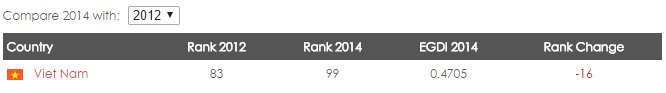
\includegraphics[scale=.85]{2014-vietnam-edgi.PNG}
    \end{center}
    \caption{Chỉ số phát triển CPĐT của Việt Nam năm 2014}
    \label{refhinh1}
    \end{figure}
\end{center}
Những khó khăn và trở ngại trong quá trình xây dựng CPĐT ở Việt Nam có thể kể đến sau đây:
\begin{itemize}
	\item[•]Cơ sở hạ tầng công nghệ thông tin ở nước ta còn yếu kém, bất cập từ các dự án công nghệ thông tin
	\item[•]Trình độ dân trí còn thấp, khó khăn trong việc sử dụng các dịch vụ của công nghệ thông tin (Web, di động,...)
	\item[•]Trình độ nhận thức và kỹ năng của cán bộ viên chức còn hạn chế, tâm lý không muốn chuyển đổi sang môi trường làm việc mới
	\item[•]Quy trình nghiệp vẫn chưa ổn định, gây khó khăn cho việc xây dựng một hệ thống toàn diện
\end{itemize}
\begin{center}
    \begin{figure}[htp]
    \begin{center}
     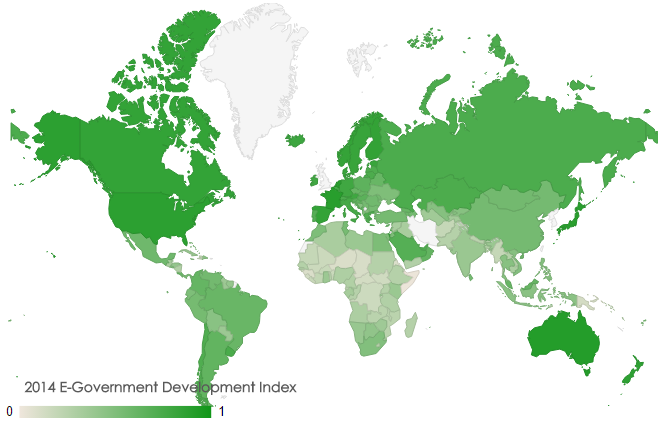
\includegraphics[scale=.8]{2014-edgi.PNG}
    \end{center}
    \caption{Chỉ số phát triển CPĐT các quốc gia năm 2014}
    \label{refhinh2}
    \end{figure}
\end{center}
Hiện nay, các dự án CPĐT đang được đẩy mạnh, nhiều cuộc tọa đàm với chủ đề công nghệ thông tin được tổ chức thường xuyên, cho thấy chính phủ ngày càng dành nhiều sự quan tâm đến việc công nghệ hóa các dịch vụ công. Ngày 14/10/2015, Chính phủ ban hành Nghị quyết số 36a/NQ-CP về Chính phủ điện tử, trong đó có một mục tiêu quan trọng là \textit{"Phấn đấu đến hết năm 2016, các bộ, ngành Trung ương có 100\% các dịch vụ công được cung cấp trực tuyến ở mức độ cho phép người sử dụng điền và gửi trực tuyến các mẫu văn bản đến cơ quan, tổ chức cung cấp dịch vụ".} Điều đó đã nêu lên được tầm quan trọng của CPĐT trong việc phát triển kinh tế, xã hội quốc gia. 
\subsection{Chi tiết về đề tài}
Nhiệm vụ chủ yếu của đề tài là xây dựng kênh tương tác 2 chiều giữa chính phủ và người dân tại địa bàn Thành phố Hồ Chí Minh, dựa trên 2 nền tảng là Web và di động. Trong đó, tương tác 2 chiều trong phạm vi của đề tài có nghĩa là:
\begin{itemize}
     \item[•]Ứng dụng cho phép người dân phản ánh các sự cố (điện, nước, giao thông,...) cho các cơ quan chức năng để họ có thể khắc phục kịp thời; duyệt xem và bình luận các phản ánh trước đó; xem các thông báo mới của chính phủ 
     \item[•]Chính phủ có thể thông báo đến người dân các tin tức về đời sống, xã hội (lịch cúp điện, công trình giao thông đang thi công,...); thu thập góp ý từ phía công dân, đưa mỗi phản ánh về các cơ quan chức năng chuyên biệt để giải quyết vấn đề, phản hồi nhanh chóng cho người dân
\end{itemize}
Môi trường làm việc:
\begin{itemize}
	\item[•]Hệ quản trị cơ sở dữ liệu: MySQL
	\item[•]Ngôn ngữ lập trình: Java, AngularJS, HTML
	\item[•]Công cụ lập trình: NetBeans, Android Studio
	\item[•]Hệ thống quản lý mã nguồn: GitHub
\end{itemize}
%%%%%%%%%%%%%%%%%%%%%%%%%%%%%%%%%
\section{Các dự án tương tự}
\subsection{Trên thế giới}

\subsection{Tại Việt Nam}

%%%%%%%%%%%%%%%%%%%%%%%%%%%%%%%%%
\section{Kiến thức nền}
\subsection{Open311}

\subsection{JPA}

%%%%%%%%%%%%%%%%%%%%%%%%%%%%%%%%%
\section{Hiện thực dự án}
\subsection{Cơ sở dữ liệu}
Từ những phân tích về các chức năng của ứng dụng, chúng em xác định cơ sở dữ liệu sẽ bao gồm bảng User quản lý các tài khoản và thông tin người dùng, bảng Request và Comment lưu trữ góp ý và bình luận của người dùng. Lược đồ Entity - Relation ship giữa các thực thể trong ứng dụng được mô tả ở Hình 3, bao gồm:
\begin{itemize}
\item[•]\textbf{Request: }Là thực thể mô tả một góp ý của người dân đến chính quyền, các thuộc tính của thực thể này bao gồm tên, mã số, địa chỉ, mô tả, hình ảnh, vị trí, id người gửi, v.v
\item[•]\textbf{Comment: }Là thực thể mô tả bình luận trong về một góp ý nào đó, có thể có nhiều bình luận trong một góp ý, các thuộc tính của thực thể bao gồm id của bình luận, thời gian gửi, nội dung và thông tin người gửi
\item[•]\textbf{User: }Là thực thể chứa thông tin của một người dùng, đây là thực thể tổng quát hóa, bao gồm hai thực thể con là \textit{người dùng thông thường (normal user)} và \textit{khách (guest).} Các thuộc tính của thực thể này bao gồm id, loại người dùng, email, tên và token của tài khoản
\item[•]\textbf{Normal User: }Là thực thể chứa thông tin của người dùng thông thường, được thừa kế từ thưc thể User, bao gồm các thuộc tính id, số CMND, mật khẩu và số điện thoại
\item[•]\textbf{Guest User: }Là thực thể chứa thông tin của khách, được thừa kế từ thực thể User, chỉ có một thuộc tính là id
\end{itemize}
\begin{center}
    \begin{figure}[htp]
    \begin{center}
     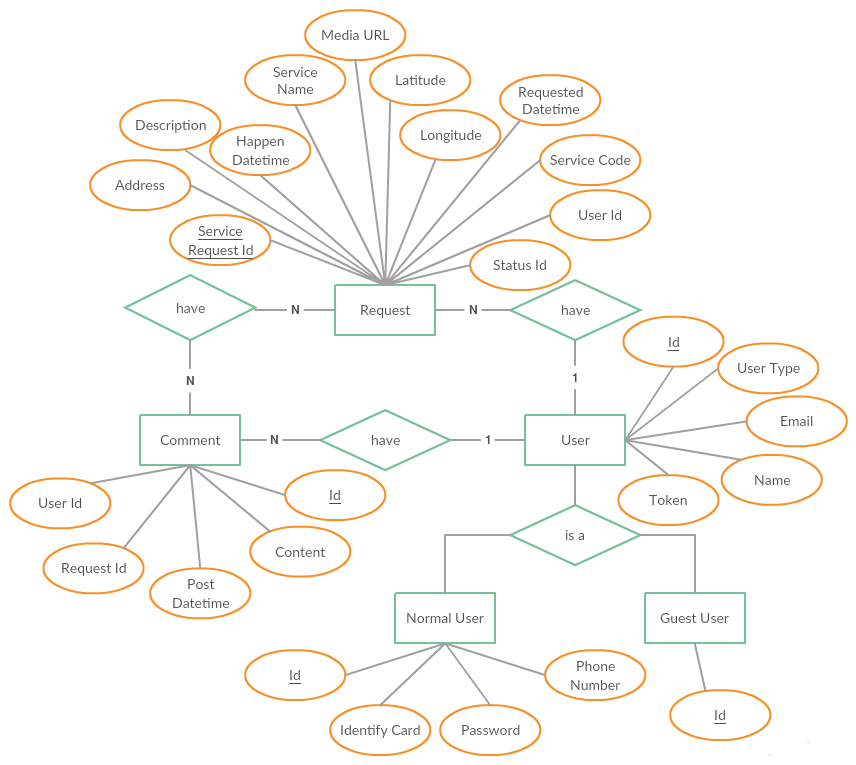
\includegraphics[scale=.65]{entity-diagram.png}
    \end{center}
    \caption{Mô hình Entity - Relationship của đề án}
    \label{refhinh1}
    \end{figure}
\end{center}
Tuy nhiên nhóm không tạo trước cơ sở dữ liệu mà sử dụng chức năng tạo ra cơ sở dữ liệu động trong lần chạy đầu tiên của ứng dụng. Việc này được thực hiện thông qua JPA API, các bảng trong cơ sở dữ liệu tương ứng với các JPA Entity đã được hiện thực trước đó.
\subsection{Client}

\subsection{Server}

%%%%%%%%%%%%%%%%%%%%%%%%%%%%%%%%%
\section{Khó khăn và khắc phục}

%%%%%%%%%%%%%%%%%%%%%%%%%%%%%%%%%
\section{Mở rộng đề tài}
Hiện tại nhóm chỉ mới phát triển ứng dụng trên nền Web. \\ 
\\
Trong giai đoạn luận văn tốt nghiệp, nhóm sẽ hoàn thành các nhiệm vụ sau:
\begin{itemize}
	\item[•]Hoàn chỉnh giao diện web cho ứng dụng
	\item[•]Tiếp tục tìm hiểu về cách làm việc của CPĐT, thủ tục hành chính của các bên liên quan để hoàn thiện các luồng làm việc của ứng dụng
	\item[•]Sửa chữa các lỗi còn tồn tại
	\item[•]Phát triển ứng dụng trên nền tảng di động
	\item[•]Viết báo cáo về đề tài
\end{itemize}
%%%%%%%%%%%%%%%%%%%%%%%%%%%%%%%%%
\section{Kết luận}
Đề án Chính phủ điện tử hiện nay là cơ hội lớn cho ngành công nghệ thông tin Việt Nam. Nhận thấy tầm quan trọng của nó, chúng em hy vọng với đề tài này, chúng em có thể góp sức vào công cuộc phát triển và áp dụng CPĐT vào thực tiễn ở địa bàn Thành phố Hồ Chí Minh \\
\\
Sau cuối, nhóm xin cảm ơn thầy cô đã hỗ trợ giải đáp các khó khăn và vướng mắc, giúp đỡ chúng em hoàn thiện sản phẩm.
\newpage

\section{Phụ lục}
\begin{thebibliography}{99}
\bibitem{bib1}
United Nation (13/01/2010). \textit{A General Framework for E-Government: Definition - Maturity Challenges, Opportunities, and Success.} Truy cập 18/05/2016 tại \url{http://www.unpan.org/Library/MajorPublications/UNEGovernmentSurvey/PublicEGovernanceSurveyintheNews/tabid/651/mctl/ArticleView/ModuleId/1555/articleId/20840/Default.aspx}

\bibitem{bib2}
World Bank (19/05/2015). \textit{Information \& Communication Technologies: e-Government.} Truy cập 18/05/2016 tại \url{http://www.worldbank.org/en/topic/ict/brief/e-government}

\bibitem{bib3}
United Nation (2014). \textit{Data Center: 2014 E-Government Development Index.} Truy cập 18/05/2016 tại \url{https://publicadministration.un.org/egovkb/en-us/Data-Center}

\bibitem{}
Tên tác giả, năm xuất bản. \textit{Tên sách.} Lần xuất bản. Thành phố: Nhà xuất bản.

\end{thebibliography}

\newpage
\section*{Phân công công việc}

    \begin{center}
        \begin{table}[h]
            \begin{tabular}{|l|l|l|l|}
            \hline
            STT & Tên & Nhiệm vụ & Đánh giá\\
            \hline
            1 & Võ Văn Luận & Xây dựng database, model, router & 100\%\\
              & &         & \\
            \hline
            2 & Trần Văn Tài & Thiết kế trang đăng nhập, đăng ký, & 100\%\\
              & & chỉnh sửa thông tin, giao diện &\\
            \hline
            \end{tabular}
        \end{table}    
    \end{center}

\listoffigures
\newpage
%%%%%%%%%%%%%%%%%%%%%%%%%%%%%%%%%

\end{document}

